\documentclass[12pt]{beamer}
%\documentclass[handout,xcolor=pdflatex,dvipsnames,table,12pt]{beamer}
\usepackage[latin1]{inputenc}
%\usepackage[T1]{fontenc}
\usepackage{amsmath} % for math AMS fonts
\usepackage{graphicx} % to include figures
\usepackage{subfigure} % to have figures in figures
\usepackage{multimedia} % to include movies
\usepackage{listings} % to display code
\usepackage{colortbl} % colored tables
\usepackage[latin1]{inputenc} % support for accented letters, etc.
\usepackage{amsthm}
\usepackage{hyperref}
\usepackage{ulem}
\usepackage{booktabs}
\usepackage{tikz}
\usepackage{mathtools}

\usetheme{Warsaw}
\setbeamercovered{invisible}

\title[Introduction to Cryptography]{Tor -- The Onion Router}
\author{Christian Mann -- christian-mann@utulsa.edu}
\institute{University of Tulsa\\
Tulsa, Oklahoma 74104}
\date{\today}

\logo{
\includegraphics[height=1.5cm]{pictures/SFSLogoMain}}

\begin{document}

\lstset{
language=python,                % choose the language of the code
%basicstyle=\footnotesize,       % the size of the fonts that are used for the code
%numbers=left,                   % where to put the line-numbers
%numberstyle=\footnotesize,      % the size of the fonts that are used for the line-numbers
%stepnumber=2,                   % the step between two line-numbers. If it's 1 each line will be numbered
%%umbersep=5pt,                  % how far the line-numbers are from the code
%backgroundcolor=\color{white},  % choose the background color. You must add \usepackage{color}
showspaces=false,               % show spaces adding particular underscores
showstringspaces=false,         % underline spaces within strings
showtabs=false,                 % show tabs within strings adding particular underscores
%%frame=single,	                % adds a frame around the code
tabsize=4,	                % sets default tabsize to 2 spaces
%%captionpos=b,                   % sets the caption-position to bottom
%%breaklines=true,                % sets automatic line breaking
%%breakatwhitespace=false,        % sets if automatic breaks should only happen at whitespace
%%title=\lstname,                 % show the filename of files included with \lstinputlisting; also try caption instead of title
%escapeinside={\%*}{*)}          % if you want to add a comment within your code
%morekeywords={*,...}            % if you want to add more keywords to the set
}

\newtheorem{mydef}{Definition}


\begin{frame}
\titlepage
\end{frame}


% no outline

% note, you should have three sections maximum.  two is good.  subsubsections are evil.
% new slides begin with teh \begin{frame} and end with \end{frame}

\iffalse
TOR: The Onion Router
Overall Idea
Key Exchange
Specifics
Attacks/Mitigations
\fi

\begin{frame}{Onion Routing}
	\begin{block}{Goals of cryptography}
		Most encryption schemes are designed to support these four properties:
		\begin{itemize}
			\item \textbf{Confidentiality} -- symmetric encryption
			\item \textbf{Integrity} -- hashes
			\item \textbf{Authenticity} -- MACs and asymmetric encryption
			\item \textbf{Non-repudiation} -- signatures
		\end{itemize}
	\end{block}

	\begin{block}{Goals of ``private'' cryptography}
		For secret routing, we need the following:
		\begin{itemize}
			\item \textbf{Anonymity}
			\item \textbf{Deniability}
			\item \textbf{Perfect Forward Secrecy}
		\end{itemize}
	\end{block}
\end{frame}

\begin{frame}{Onion Routing}
	\begin{block}{Problem}
		Network traffic can be sniffed, snooped, and monitored. While protocols
		like TLS give end-to-end secrecy, they do not prevent an eavesdropper
		from discovering \textit{who} is communicated with \textit{whom}, and at
		what times.
	\end{block}
	\begin{block}{Goal}
		We would like to anonymize traffic, so that no  eavesdropper can
		determine the source of any given connection.
	\end{block}
\end{frame}

\begin{frame}{Onion Routing}
	\begin{block}{Adversary}
		In academic papers, a \textbf{global passive} adversary is considered,
		one that can monitor all traffic on all links at all times.

		Tor is \textbf{not} designed against this adversary model. Instead it
		assumes an adversary who can
		\begin{itemize}
			\item Observe some fraction of network traffic;
			\item Generate, modify, delete, or delay traffic;
			\item Operate onion routers of his own;
			\item Compromise some fraction of the onion routers.
		\end{itemize}
	\end{block}
\end{frame}

\begin{frame}{Tor}{Design}
	\begin{block}{Overview}
		\begin{itemize}
			\item Network of ``onion routers'' across the Internet
			\item Listed on a directory server
			\item Each onion router (OR) securely connects to others via TLS
			\item User runs onion proxy (OP), a SOCKS proxy
			\item The OP accepts TCP connections and spreads them over the
				network
			\item The last onion router connects to the destination and sends
				data
			\item Overall resembles a \textit{circuit-switched} network
		\end{itemize}
	\end{block}
\end{frame}

\begin{frame}{Tor Design}{Details}
	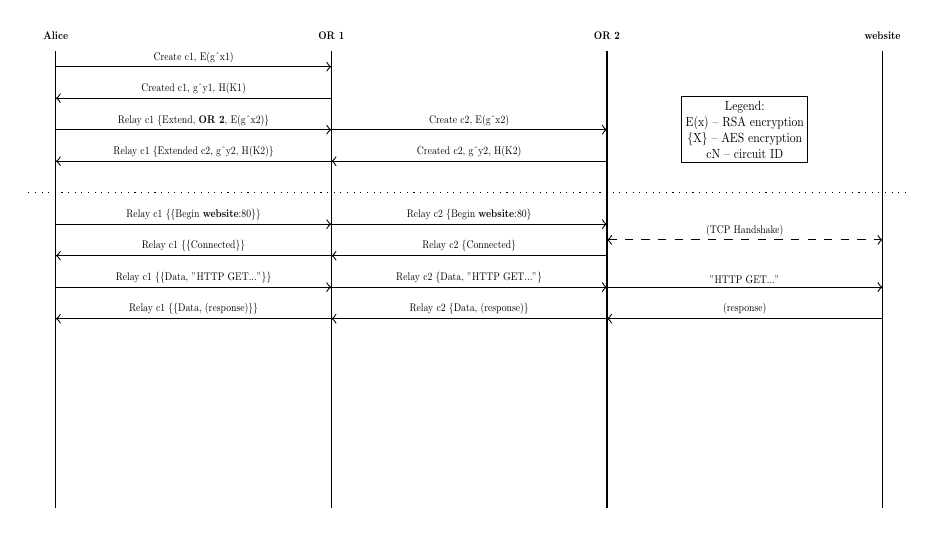
\begin{tikzpicture}[xscale=0.35, yscale=0.4, every node/.append style={transform shape}]
		\node at (0,0) {\bf Alice};
		\node at (10,0) {\bf OR 1};
		\node at (20,0) {\bf OR 2};
		\node at (30,0) {\bf website};

		\draw (0,-0.5) -- (0,-15);
		\draw (10,-0.5) -- (10,-15);
		\draw (20,-0.5) -- (20,-15);
		\draw (30,-0.5) -- (30,-15);

		\draw [->] (0,-1) -- (10,-1) node[above,midway] {Create c1,
		E(g\^{}x1)};
		\draw [->] (10,-2) -- (0,-2) node[above,midway] {Created c1, g\^{}y1,
		H(K1)};
		\draw [->] (0,-3) -- (10,-3) node [above,midway] {Relay c1 \{Extend,
		\textbf{OR 2}, E(g\^{}x2)\}};
		\draw [->] (10,-3) -- (20,-3) node [above,midway] {Create c2,
		E(g\^{}x2)};
		\draw [->] (20,-4) -- (10,-4) node [above,midway] {Created c2, g\^{}y2,
		H(K2)};
		\draw [->] (10,-4) -- (0,-4) node [above,midway] {Relay c1 \{Extended
		c2, g\^{}y2, H(K2)\}};
		\draw [dotted] (-1,-5) -- (31,-5);
		
		\draw [->] (0,-6) -- (10,-6) node [above,midway] {Relay c1 \{\{Begin
		\textbf{website}:80\}\} };
		\draw [->] (10,-6) -- (20,-6) node [above,midway] {Relay c2 \{Begin
		\textbf{website}:80\}};
		\draw [<->,dashed] (20,-6.5) -- (30,-6.5) node [above,midway] {(TCP Handshake)};

		\draw [->] (20,-7) -- (10,-7) node [above,midway] {Relay c2 \{Connected\}};
		\draw [->] (10,-7) -- (0,-7) node [above,midway] {Relay c1
		\{\{Connected\}\}};

		\draw [->] (0,-8) -- (10,-8) node [above,midway] {Relay c1 \{\{Data,
		"HTTP GET..."\}\}};
		\draw [->] (10,-8) -- (20,-8) node [above,midway] {Relay c2 \{Data,
		"HTTP GET..."\}};
		\draw [->] (20,-8) -- (30,-8) node [above,midway] {"HTTP GET..."};
		\draw [->] (30,-9) -- (20,-9) node [above,midway] {(response)};
		\draw [->] (20,-9) -- (10,-9) node [above,midway] {Relay c2 \{Data,
		(response)\}};
		\draw [->] (10,-9) -- (0,-9) node [above,midway] {Relay c1 \{\{Data,
		(response)\}\}};

		\node [draw,align=center,scale=1.2] at (25,-3) {Legend:\\E(x) -- RSA
		encryption\\ \{X\} -- AES encryption \\ cN -- circuit ID};
	\end{tikzpicture}
\end{frame}

\begin{frame}{Tor Design}{Important Properties}
	\begin{itemize}
		\item \textbf{Ephemeral} Diffie-Hellman keys are exchanged with each
			hop.
		\item The DH exchange is \textbf{authenticated} with the OR's public
			key.
		\item Each relay does not know the original host, nor the final
			destination.
		\item Circuits can be of arbitrary topology.
		\item Each node has the ability to refuse a connection to the next node.
			This does not impede the network.
	\end{itemize}
\end{frame}

\begin{frame}{Tor Design}{Integrity Checking}
	\begin{block}{Problem -- Integrity and Replay}
		When Alice negotiates a key with a new hop, the two ends initialize a
		SHA-1 digest with a derivative of that key. Each ``cell'' (packet) is
		fed into that hash, and tagged with the current state of the hash.

		Any modification can be thus detected, including replay attacks.
	\end{block}
\end{frame}

\begin{frame}{Attacks on Tor}
	\begin{itemize}[<+->]
		\item Exit node eavesdropping
		\item Path Takeover
		\item Overall traffic analysis -- what goes in comes out
		\item Traffic analysis attack -- coordinating traffic to same originator
		\item Tor exit node block
		\item IP Address disclosure via e.g. BitTorrent
		\item Bad Apple Attack -- discovering traffic from a known IP address
		\item ``Sniper attack'' -- fill exit nodes' buffers
		\item Any TLS attack e.g. Heartbleed
	\end{itemize}
\end{frame}

\begin{frame}{Questions / Comments?}
\end{frame}

\end{document}
